%===================================================================================================
%  Chapter : 運動の法則と万有引力
%  説明    : ニュートンの運動の3法則・万有引力の法則について,説明する.
%===================================================================================================
\begin{mycomment}
    ニュートン力学は,4つの法則により成立している.
    4つの法則のうち,3つは物体の運動に関する法則(運動の3法則といわれる)であり,
    残りの1つは万有引力の法則である.
    物体は,この4つの法則を満たすように運動する.
    この章では,
    ニュートンの運動の3つの法則,万有引力の法則を説明していく.
\end{mycomment}
%   %==========================================================================
%   %  Section
%   %==========================================================================
    \section{運動の3法則}
%       %======================================================================
%       %  SubSection
%       %======================================================================
  \subsection{(第1法則)慣性の法則}
                力を与えられていない物体は,その動き方に変化は生じない.
                外力が加わらなければ,等速直線運動している物体は等速直線運動を続けるし,
                静止している物体は静止し続ける.
                このような性質を物体の運動の根本原因と考え,法則と捉える.
                この法則の名前を \textbf{慣性の法則} という
                \footnote{
                  「…し続ける」という性質を,\textbf{慣性} という.
                }.

                慣性の法則は実験によってのみ確かめることができ,
                どのような原理でこの法則が成立しているのかということを問題とはしない
                  \footnote{
                    問題にすることはできない,と言ったほうがよい.物理学は自然現象を論理的に説明
                    する学問である.論理的説明をするには,説明なしに受け入れなければいけない約束事
                    を設ける必要がある.これを数学では \textbf{公理} というが,物理学でこの公理
                    に対応するものが \textbf{法則} と言われるものである.
                    慣性の法則は,このような説明なしに受け入れるべき法則の1つである.
                  }.

                まとめておこう.
                \begin{myshadebox}{慣性の法則}
                    物体の運動に関する次のような性質を,\textbf{慣性の法則} という.
                    \begin{itemize}
                        \item 座標系 $S$ に対して静止している物体は,
                              外力が加わらない限り,$S$ に対して静止し続ける.
                        \item 座標系 $S$ に対して速度をもっている物体は,
                              外力が加わらない限り,$S$ に対してその速度を保ち続ける.
                    \end{itemize}
                \end{myshadebox}
                \begin{figure}[hbt]
                    \begin{center}
                        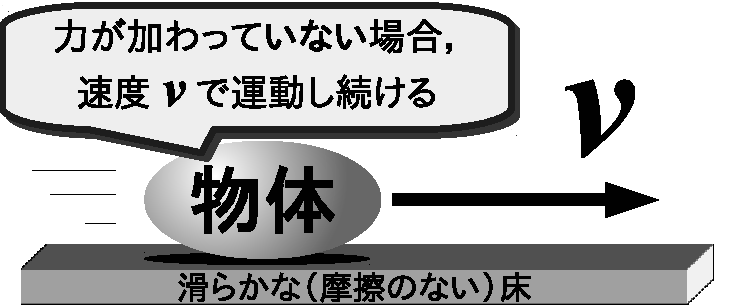
\includegraphics[keepaspectratio, width=4.8cm,height=2.0cm,clip]{kanseinohousoku.pdf}
                        \caption{慣性の法則}
                        \label{fig:kanseinohousoku}
                    \end{center}
                \end{figure}

                この法則によって,慣性系の存在が暗黙的に仮定される
                    \footnote{
                        もっとストレートに「慣性系が一つ存在する」と表せばよいのだが,どの教科書を見ても,
                        何故か,そう書かれていない.このノートもその例に従っている.
                        確かに,等速運動を続けるとか静止し続けると書いたほうが,直感的にわかりやすい.
                    }.
                「速度をもつ」とか「加速度をもつ」とかという場合,基準となる慣性系が必要だからである.
                相対速度の項目で確認したように,観測者の見る物体の速度は,
                観測者と物体間の相対速度である.すなわち,同じ物体を見ているのにもかかわらず,
                別の速度で運動している観測者にっとっては,物体は全く異なった速度として観測される.
                極端な例では,物体と同じように等速直線運動する座標系から物体を見た場合は,
                その物体は静止しているとみなされる.つまり,座標系によって物体の速度が異なってしまう.
                そこで,等速直線運動する全座標系から一つ基準となる慣性系を選び,
                この座標系を特別な座標系として扱うのが最も自然である.
                選び出された1つの座標系は速度をもっていないとみなされ
                  \footnote{
                    基準となる座標系に速度がなければ,理論的に整った(補正項のいらない)説明ができる.
                    その他の座標系は,この基準となる座標系に補正項を加えた形で表現することができる.
                  },
                これは \textbf{絶対静止系} とよばれる.

                上記の慣性の法則で言っている座標系 $S$ とは,絶対静止系のことである.
                力学は絶対静止系を,速度や加速度,力の基準として構築されている
                    \footnote{相対性理論によると,絶対静止系 $S$ の存在は否定されるが,
                        ニュートン力学を考える範囲では系 $S$ の存在を仮定したうえで成立する
                        理論である.認めてもその理論に支障はない.
                    }.

                以下では,単に速度とか加速度とかと書いた場合は,それは系 $S$ に対するもの
                であると考える.
                ちなみに,車や電車の速度の基準は,地球を基準(絶対静止系)とした場合のものである
                  \footnote{
                    地球は太陽の周りを公転しているので静止していないではないか,という反論が
                    あるかもしれないが,実際には私達は地球が静止しているように感じており,こう考えても
                    実使用上は問題はない(物理理論的には問題だが,工学的には有効な考え方である).
                    絶対静止系を任意に取れることを身近な例によって示したかったので,地球を例にした.
                  }.

                絶対静止系は等速直線運動している全座標系から任意にひとつだけ選びとった座標系であるので,
                等速度運動状態と静止状態が全く同等である.

                逆に,物体の動き方が変わった時(加速度が生じた場合)には,力が作用したと考える
                具体的には運動の第2法則(運動方程式)として記述される.
                物体に力が加わった場合,その物体は加速度が生じる.

%       %======================================================================
%       %  SubSection
%       %======================================================================
        \subsection{(第2法則)運動方程式}
                運動の第2法則は実際に動いている物体に対するものである.具体的には,
                重い物体は動かしにくく,軽い物体は動かしやすい.このようなイメージを
                式で表現する.

                物体の運動は以下の式によって記述できる.
                    \begin{align}\label{undouhouteisiki}
                        \frac{\df^{2}\br}{\df t^{2}} = k\frac{\bF}{m_{\mathrm{i}}}
                    \end{align}
                ここで,$k$は定数,$m_{\mathrm{i}}$ は \textbf{慣性質量} であり,
                $\bF$ は力 である.言葉でいうと,
                    \begin{center}
                『物体の加速度は 慣性質量に反比例し,力に比例する』
                    \end{center}
                である.これを \textbf{運動方程式} という.

                おそらく,歴史的には紆余曲折があって,最終的にこの形に落ち着いたのであろう.
                ニュートンが提示した最初の式は,微分積分学が整っておらず
                  \footnote{
                    ニュートンのこの力学の提示で,微分積分学が始まったとすれば,当然だ.
                    微分方程式という考え方はニュートンの力学以降に発展するのであり,
                    また,よりよい式表現のための記号法が整備されることになる.
                  },
                当然ながらこのような微分方程式の記述にはなっていなかったはず.
                式の形がこうなるまでの経緯は歴史的には重要かもしれないが,
                このノートでは興味のないことである.すでに数式的に整った形になっているのだから,
                これを積極的に受け入れるべきである.同じニュートンの運動法則を意味している
                のには変わりないのだから.

                運動方程式をもう少し整理し,わかりやすく書き換えよう.
                力の単位 $[\rm{N}]$ を$[\rm{N}] = [\rm{kg (m/s^{2})}]$ すると,
                定数$k$は $k=1$ になって,以下のように書ける.
                        \begin{myshadebox}{運動方程式}
                            ニュートンの運動方程式は,以下のように表現される.
                            \begin{align}\label{eq:N_eq}
                            m_{\rm{i}}\frac{\df^{2}\br}{\df t^{2}} = \bF
                            \end{align}
                        \end{myshadebox}
                        \begin{figure}[hbt]
                            \begin{center}
                                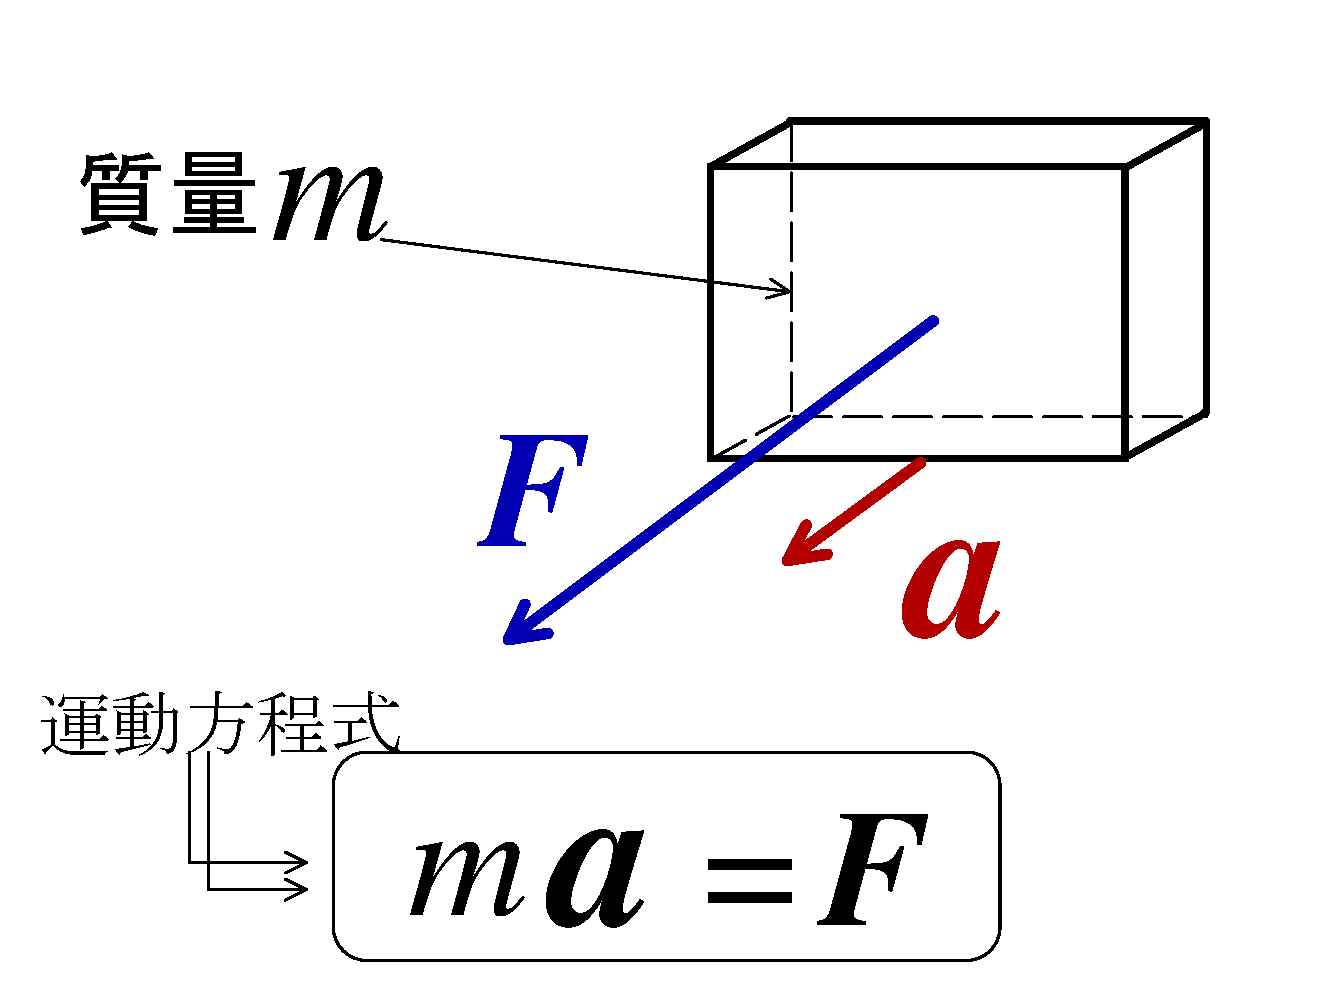
\includegraphics[keepaspectratio, width=6cm,height=6cm,clip]{ma_F.pdf}
                                \caption{運動方程式}
                                \label{fig:ma_F}
                            \end{center}
                        \end{figure}

                加速度は力に比例するので,その比例係数を慣性質量 $m_{\mathrm{i}}$ と見るのである
                    \footnote{
                        もともとあった比例定数 $k=1$ の記述は省略するが,
                        その理由が力の単位の取り方にあるということは覚えておくべきである.
                        これ以降でも様々な物理法則を表す式を見ていくが,比例定数が現れない
                        ことが多い.
                        これは理論的説明を簡潔に表現するべく,物理量の単位の定義を人為的に都合よく行っているからである.

                        単位の取り方によって,数値は変わってしまう(時には次元そのものも変わりうる)が,
                        これは物理的現象の本質ではない.物理現象を人間が説明しようとするときには,
                        ある視点からその現象を観測する必要がある.
                        観測するということは,その対象となる物理現象を偏った考えの下で見るということである.
                        こうなると当然ながら,同じ現象でも,観測方法の違いによって,測定結果がことなる場合が起こる.
                        しかし,間違いはどこにもない.どちらも正しい.同じ現象なのに,
                        測定方法によって異なる結果が出るのはおかしな気がするかもしれないが,受け入れるしかない.
                        1つの物理現象に対して,複数の物理学的説明があってもよいではないか.
                        理論は1つだけとは限らないの(人間は本当の物理法則を知ることはできない)と
                        考えるほうが健全な思考である.
                        このことは,学習を進めていくうえで忘れがちなので,ここで注意を促しておいた.
                    }.
                そうすれば「物体の質量が大きいほど,その物体に加速度をもたせるために必要な力は,
                大きくなる」と読み取れる.
                (力と加速度に具体的な数値を代入して確認してみるとよい.)
                すなわち,慣性質量は,「物体の動きにくさ」を表現していると考えられる.
                以下では,運動方程式として,式(\ref{eq:N_eq}) を用いることにする.

                運動方程式(\ref{eq:N_eq})は,慣性質量と加速度と力の3つの概念の関係を
                示しているだけであり,力の定義をなしているわけではないことに注意する.
                ここでは,とりあえず,「力」というものの存在を仮定しているのである.

                この法則で使われる等号は数学的に厳密な等号ではない.
                この法則は実験によって得られるものだからである.
                例えば,実験で加速度や慣性質量や力を
                測定するとき,必ず測定限界となる桁数が存在する.
                つまり,無限桁だけの測定はできないのだから,
                「ニュートンの運動方程式は小数点第○位の桁で正しい」としかいえない.
                すなわち,ニュートンの運動方程式(ニュートン方程式)における等号は,
                細かくいえば,近似を表すものである.
                しかし,物理では等号のようにして扱う.これによる不都合は
                ほとんどない.不都合が現れるのは量子力学や相対性理論で
                考える状況下においてである
                    \footnote{
                        相対性理論;光速に近い速度で動く物体を考える(特殊相対性理論).
                        一様でない重力が存在する空間を考える(一般相対性理論).
                        量子力学;原子レベルの大きさの粒子の運動の記述を考える.
                    }.
                そのときはニュートン方程式
                を書き換えてやればよい.このニュートン方程式は
                私達の目に見える物体の動きを
                かなりの精度で正確に記述できる方程式である.

%       %======================================================================
%       %  SubSection
%       %======================================================================
        \subsection{(第3法則)作用$\cdot$反作用の法則}
            2つの物体をもってきて,それぞれ名前をA,Bとする.
            このとき,\textbf{作用反作用の法則}とは以下のような法則のことである.
                \begin{myshadebox}{作用反作用の法則}
                    『物体Bが物体Aに力$\bF_{\rm{AB}}$を与えているとき,
                    物体Aも物体Bに$\bF_{\rm{AB}}$と大きさが同じで逆向きの力
                    $-\bF_{\rm{BA}}$を受けている』
                \end{myshadebox}
            \begin{figure}[hbt]
                \begin{center}
                    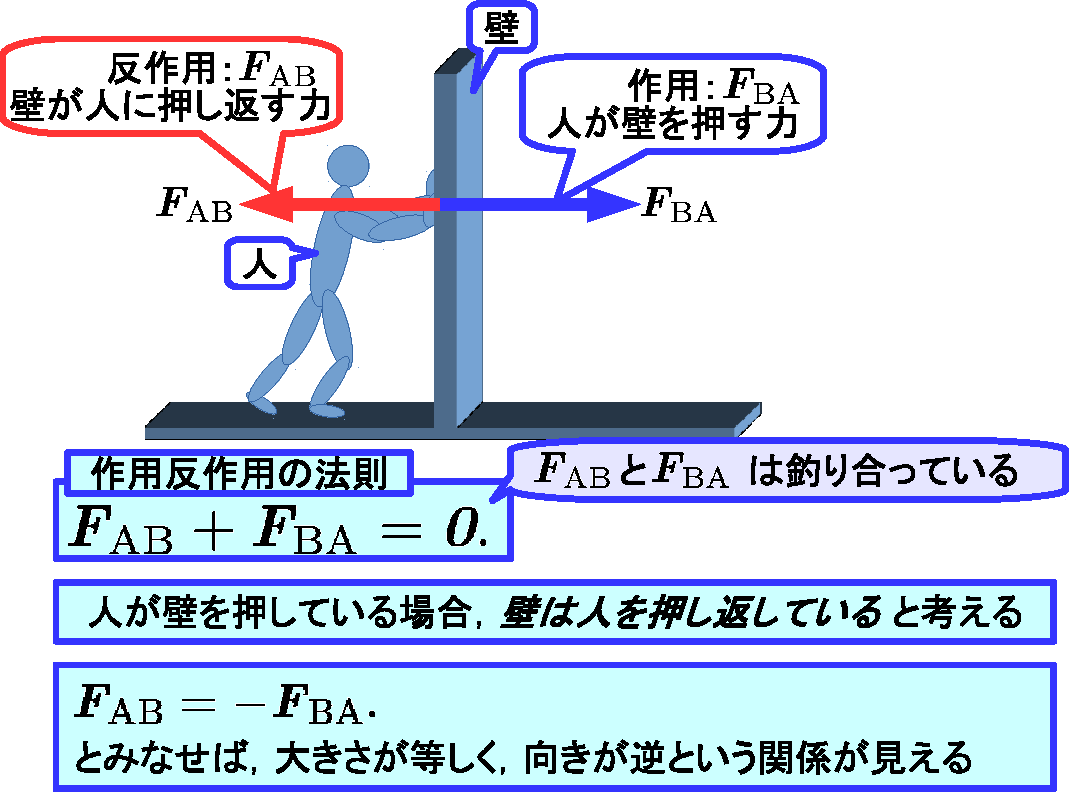
\includegraphics[keepaspectratio, width=6cm,height=6cm,clip]{sayou_hansayou.pdf}
                    \caption{作用$\cdot$反作用の法則}
                    \label{fig:sayou_hansayou}
                \end{center}
            \end{figure}

            これを式で表すと,
                \begin{align}
                    \bF_{\mathrm{AB}} = -\bF_{\mathrm{BA}}
                \end{align}
            である.この式を変形すると,
                \begin{align}
                    \bF_{\mathrm{AB}} +\bF_{\mathrm{BA}}= 0
                \end{align}
            となって,作用とその反作用で生じる力からの合計は 0 になることがわかる.
            作用とは,ここでは,力のことをいう.

            力いっぱい押してもビクともしない壁を,
            力いっぱい押してみよう.しかし,壁は動かない.
            壁に力を加えているのにその壁が動かないということは,
            ニュートン方程式に反していると,一見して見まちがえ得る.
            しかし,作用反作用の法則による,壁に押し返されていることを
            考えれば矛盾でもなんでもない.

            この法則は,「力」のもつ性質を記述している.
            この法則の対象は「力」そのものである.
            しかし,今までに「力」を明確に定義していないので,
            少々曖昧に聞こえてしまうかもしれない.
            実際,その通りである.この作用反作用の法則は他の2つの法則より
            も,何か違った雰囲気がある.この法則は
            「力とは何か」が分かったときに,
            削除されるものなのかもしれない.
            しかし,ここではそんな高度な質問に
            答えることは不可能であり,
            さしあたってはこの法則を受け入れて
            いくことにしよう.

            そうはいうものの,この法則は大切な法則である.
            この法則によって,物理学で重要な概念の1つである,
            保存則が導かれるからである.「保存する」とは時間に関係なく
            一定の値をとることをいう.
            保存則については後ほど詳しく考えていきたい.
            ここでは,作用反作用の法則は捨ててはならない重要な
            法則であるということをわかればそれでよい.

%       %======================================================================
%       %  SubSection
%       %======================================================================
        \subsection{慣性質量}
                運動方程式(第2法則)で現れた質量を \textbf{慣性質量} という.
                これは,すぐ後に説明する万有引力の法則に現れる質量
                    \footnote{
                        こっちは \textbf{重力質量} とよぶことになるが,詳細は後に述べる.
                    }
                と区別するための名前である.慣性質量の大きさの比べ方について,ここで
                学習しておこう.

                2つの質量があるとしよう.これらを $m_{i1}$,$m_{i2}$ とおく.
                この2つの質量に全く同じ力 $F$ を加えて,それぞれに加速度を与える.
                向きはあまり本質的でないので省略する.
                加速度が生じることは式(\ref{undouhouteisiki})によって保証されている.
                このときの各質点の加速度は,加わる力が一定でも質量が異なるので,
                互いに異なったものとなる.簡単のために,二つの質点は同一方向に
                運動するとしよう.各質点の加速度の大きさを $a_{1}$,$a_{2}$ とする.
                ここで加速度の向きも省略する.
                運動方程式(\ref{undouhouteisiki})によって,各質点の運動は以下のように記述される.
                    \begin{equation*}
                        a_{1}=k\frac{F}{m_{i1}}\,,\quad a_{2}=k\frac{F}{m_{i2}}
                    \end{equation*}
                この2つの式から共通の $F$ を消去すると以下の関係を得る.
                    \begin{equation*}
                        (kF=)\;a_{1}m_{i1}=a_{2}m_{i2}
                    \end{equation*}
                    \begin{equation*}
                        \frac{a_{1}}{a_{2}}=\frac{m_{i1}}{m_{i2}}
                    \end{equation*}
                慣性質量はこのように測定される.何か基準となる質量を1つ定めることによって,
                その他の質量を決定できる.キログラム原器の1[kg]が,その基準である.

                \begin{memo}{慣性の法則と運動方程式の関係}
                    運動方程式(\ref{eq:N_eq})は,慣性質量と加速度と力の3つの概念の関係を
                    示しているだけであり,力の定義をなしているわけではないことに注意する.
                    ここでは,とりあえず,「力」というものの存在を仮定しているのである.

                    この法則で使われる等号は数学的に厳密な等号ではない.
                    この法則は実験によって得られるものだからである.
                    例えば,実験で加速度や慣性質量や力を
                    測定するとき,必ず測定限界となる桁数が存在する.
                    つまり,無限桁だけの測定はできないのだから,
                    「ニュートンの運動方程式は小数点第○位の桁で正しい」としかいえない.
                    すなわち,ニュートンの運動方程式(ニュートン方程式)における等号は,
                    細かくいえば,近似を表すものである.
                    しかし,物理では等号のようにして扱う.これによる不都合は
                    ほとんどない.不都合が現れるのは量子力学や相対性理論で
                    考える状況下においてである
                        \footnote{
                            相対性理論;光速に近い速度で動く物体を考える(特殊相対性理論).
                            一様でない重力が存在する空間を考える(一般相対性理論).
                            量子力学;原子レベルの大きさの粒子の運動の記述を考える.
                        }.
                    そのときはニュートン方程式
                    を書き換えてやればよい.このニュートン方程式は
                    私達の目に見える物体の動きを
                    かなりの精度で正確に記述できる方程式である.
                \end{memo}



%   %======================================================================
%   %  Section
%   %======================================================================
        \section{万有引力の法則}
            \subsection{法則のイメージと数式による定義}
            万有引力の法則は,ニュートンの運動の3法則とは独立したものである.
            その内容は「2つの重力質量が存在しているとき,その両者は引き合う」というものである
                \footnote{
                    「重力質量」といったのは,先ほどニュートン方程式の部分で確認した
                    慣性質量とは別に定義される質量であることを示したかったからである.
                }.
            これはすなわち,2つのうちの一方の重力質量($m_{\rm{gA}}$ としよう)が他方の
            重力質量($m_{\rm{gB}}$ としよう)を
            引っ張るのである.もちろん,反対を考えれば,
            重力質量 $m_{\rm{gB}}$ が重力質量 $m_{\rm{gA}}$ を引っ張っていることになる.
            \begin{figure}[hbt]
                \begin{center}
                    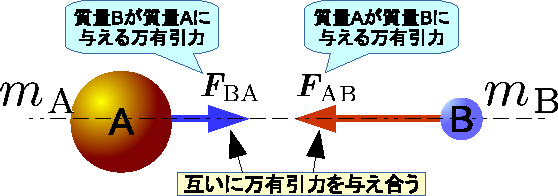
\includegraphics[keepaspectratio, width=7.2cm,height=6.64cm,clip]{bannyuuinnryoku.pdf}
                    \caption{万有引力}
                    \label{fig:bannyuuinnryoku}
                \end{center}
            \end{figure}

            以上のことを,もう一度もう少しかしこまった言い方で確認しておこう.
            2つの重力質量 $m_{\rm{gA}}$,$m_{\rm{gB}}$ が存在すると,その重力質量
            同士が互いに引き合う.
            これが \textbf{万有引力の法則} である.
            以下の式は 重力質量 $m_{\rm{gA}}$が,重力質量 $m_{\rm{gB}}$ に引っ張られる力を表す.
            力と重力質量 の添え字に注意すること.
                \begin{myshadebox}{万有引力の法則}
                    万有引力(重力質量 $m_{\rm{gA}}$が,重力質量 $m_{\rm{gB}}$ に引っ張られる力)
                    は次式で定義される.
                    \begin{align}\label{Grav}
                        \bF_{\rm{AB}}
                        = -G\frac{m_{\rm{gA}}m_{\rm{gB}}}{{\left| \br_{A}
                        -\br_{B} \right|}^{2}}
                        \frac{\br_{A}-\br_{B}}{\left| \br_{A}
                        -\br_{B} \right|}.
                    \end{align}
                    ここに,$\br_{A}$,$\br_{B}$は,それぞれ$m_{\rm{gA}}$と$m_{\rm{gB}}$の 位置である.
                \end{myshadebox}

                \begin{figure}[hbt]
                    \begin{center}
                        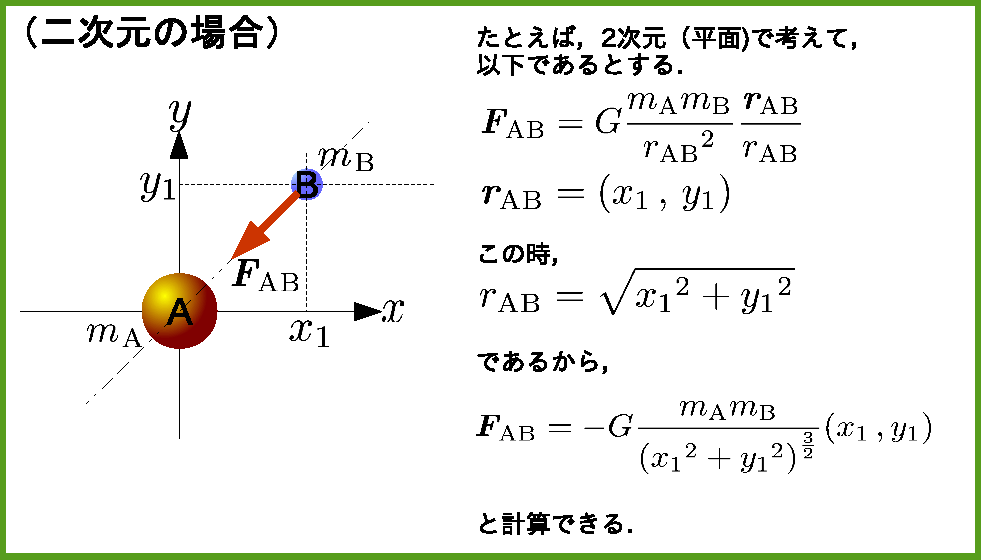
\includegraphics[keepaspectratio, width=6.5cm,height=4.2cm,clip]{bannyuuinnryoku_rei2d.pdf}
                        \caption{万有引力(例:2次元)}
                        \label{fig:bannyuuinnryoku_rei2d}
                    \end{center}
                \end{figure}

            \begin{memo}{万有引力法則とケプラーの法則}
                ニュートンが万有引力の法則を見つけたのは,
                \textbf{ケプラーの惑星の運動の3法則} を
                説明するためであった.たしかに,
                万有引力をニュートンの運動の3法則を
                用いると,ケプラーの法則が満たされる.
                逆に,ケプラーの法則から万有引力を
                導ける.どちらを基本法則としてもよいと
                思われるが,ここは万有引力を
                基本法則としたほうが無難だろう---
                ケプラーの法則は3つであり,
                万有引力は1つであるから…これも思考経済だ---
            \end{memo}

            \subsection{重力質量}
            万有引力の法則で表される質量のことを,\textbf{重力質量} という.
            重力質量は,運動方程式で表される慣性質量とは,別の概念である.
            重力質量は物体の「重さ」を表現していると考えられる
                \footnote{
                    慣性質量とは,物体の動きにくさ を表すものであった.
                }.
            また,重力質量$m_{\rm{gB}}$が 重力質量$m_{\rm{gA}}$に引っ張られる力 $\bF_{\rm{BA}}$ は
                \begin{align}
                    \bF_{\rm{BA}}
                    =-G\frac{m_{\rm{gB}}m_{\rm{gA}}}{{\left| \br_{B}
                    -\br_{A} \right|}^{2}}
                    \frac{\br_{B}-\br_{A}}{\left| \br_{B}
                    -\br_{A} \right|}
                \end{align}
            である.
            $\bF_{\rm{AB}}$ と $\bF_{\rm{BA}}$ の関係は,明らかに
            ($\br_{B}-\br_{A}$の部分に注目)
                \begin{align}
                    \bF_{\rm{AB}}=-\bF_{\rm{BA}}
                \end{align}
            であることがわかり,作用反作用の法則が成立していることも確認できる.

            \begin{memo}{この世界にある「力」の種類}
            万有引力は基本的な力の1つである.基本的な力はこの他に3つあって,
            それは「電磁気的な力」,「弱い力」,
            「核力」である.力のことを \textbf{相互作用} ということもある.

             古典力学でいう力とは, 主に,電磁気的な力 と 万有引力 である.
            \end{memo}

            \subsection{重力加速度}
                万有引力の法則は,2つの物体間に関する法則である.
                ここで,違う視点から,万有引力の法則を眺めてみる.
                物体の一つを惑星,もう一方を任意の物体と考えてもらいたい.
                物体が惑星に引っ張られているイメージ.

                惑星の質量を,$M_{P}$,惑星の位置を $\br_{P}$ とする.
                    \footnote{
                        添字の $P$ は Planet の頭文字.
                    }.
                また,惑星上の物体の質量を $m_{\mathrm{g}}$,位置を $\br$ とする.

                すると,物体が惑星から受ける力は,以下の式で表せる.
                    \begin{equation*}
                        \bF
                        =-m_{\mathrm{g}}\left( G\frac{M_{P}}{{\left| \br-\br_{P} \right|}^{2}}
                        \frac{\br-\br_{P}}
                        {\left| \br-\br_{P}\right|}\right).
                    \end{equation*}
                ここに,$\br$,$\br_{P}$ はそれぞれ,質点の位置 と 惑星の位置 を表す.

                今基準としているのは惑星だから,惑星の位置を基準にすれば($\br_{P}=\bzero$),
                    \begin{equation*}
                        \bF
                        =-m_{\mathrm{g}}\left( G\frac{M_{P}}{{\left| \br \right|}^{2}}
                        \frac{\br}
                        {\left| \br\right|}\right).
                    \end{equation*}

                ここで,\textbf{重力加速度} を以下で定義する.
                        \begin{myshadebox}{重力加速度の定義}
                            次式で,重力加速度を定義する.
                            \begin{align}\label{eq:GravAccer000}
                                \textit{\textbf{g}} :=
                                G\frac{M_{P}}{{\left| \br \right|}^{2}}
                                \frac{\br}{\left| \br \right|}.
                            \end{align}
                        \end{myshadebox}

                万有引力の法則に,惑星の質量 $M_{P}$,惑星の位置 $\br_{P}=\bzero$ を代入している.
                この定義において,重力加速度の向きは惑星から質点に向かう方向である.従って,鉛直上向きを正とする.
                この重力加速度は惑星の近くではほぼ一定であるとみなせる.従って,惑星の表面付近から受ける力は,重
                力加速度を用いて,
                    \begin{align}
                        \bF =- m_{\mathrm{g}}\textit{\textbf{g}}
                    \end{align}
                と書ける.すなわち,質点は地表よりも上に存在するとき
                    \footnote{
                        地表:地球の表面のことをいう.
                    },
                質点は惑星に向かう方向に重力を受けることになる.負の符号が付いている理由は,
                惑星から質点に向かう方向を正方向にとっているため.
